\documentclass{article}


%preamble
%required
%\usepackage{Sweave} %Integrates R code with LaTeX for creating dynamic reports
\usepackage{natbib}%Provides citation and bibliography support
\usepackage{amsmath}%Enhances mathematical typesetting capabilities.
\usepackage{textcomp}%among other things, it allows degrees C to be added
\usepackage{float}%Helps with precise figure placement using the [H] option.
\usepackage[utf8]{inputenc} % allow funny letters in citations 
\usepackage[nottoc]{tocbibind} %should add Re fences to the table of contents?
\usepackage{amsmath} % making nice equations 
\usepackage{listings} % add in stan code
\usepackage{xcolor}
\usepackage{capt-of}%allows me to set a caption for code in appendix 
\usepackage[export]{adjustbox} % adding a box around a map
\usepackage{lineno}
\linenumbers

\usepackage[margin=2cm]{geometry}
\usepackage[most]{tcolorbox}

\newtcolorbox{mytextbox}[1][]{% specify textbox
	sharp corners,
	enhanced,
	colback=white,
	height=15cm,
	attach title to upper,
	#1
}

% recommended! Uncomment the below line and change the path for your computer!
% \SweaveOpts{prefix.string=/Users/Lizzie/Documents/git/teaching/demoSweave/Fig.s/demoFig, eps=FALSE} 
%put your Fig.s in one place! Also, note that here 'Fig.s' is the folder and 'demoFig' is what each 
% Fig. produced will be titled plus its number or label (e.g., demoFig-nqpbetter.pdf')
% make your captioning look better
\usepackage[small]{caption}

\usepackage{xr-hyper} %refer to Fig.s in another document
\usepackage{hyperref}

\setlength{\captionmargin}{30pt}
\setlength{\abovecaptionskip}{0pt}
\setlength{\belowcaptionskip}{10pt}

% optional: muck with spacing
\topmargin -1.5cm        
\oddsidemargin 0.5cm   
\evensidemargin 0.5cm  % same as odd side margin but for left-hand pages
\textwidth 15.59cm
\textheight 21.94cm 
% \renewcommand{\baselinestretch}{1.5} % 1.5 lines between lines
\parindent 0pt		  % sets leading space for paragraphs
% optional: cute, fancy headers
\usepackage{fancyhdr}
\pagestyle{fancy}
%\fancyhead[LO]{Frederik Baumgarten}
%\fancyhead[RO]{Research Proposal}
% more optionals! %

\usepackage{graphicx}
\graphicspath{{/Users/frederik/github/PlantDeterminism/figures/}} % specify the path to your figures directory




\begin{document}
	
	
	\title{Invest now, get paid later? Growth strategies to cope with environmental stress and benefit from extended growing seasons in a future climate %(my favourite)
		
		%dlDec18: Alternate title ideas:
		%Growth determinism/determinacy/habits in plants/woody perennials/trees: Limits and opportunities of species to time growth activities in a future climate. 
		
		%Growth determinacy in temperate trees: investing at the right time to cope with environmental stress and benefit from extended growing seasons in a future climate.
	} 
	
	\date{\today}
	\author{Frederik Baumgarten\textsuperscript{1,2}, Yann Vitasse\textsuperscript{2}, Sally?, Rob?, EM Wolkovich\textsuperscript{1}}
	\maketitle
	
	$^1$ Department of Forest and Conservation, Faculty of Forestry, University of British Columbia, 2424 Main Mall
	Vancouver, BC Canada V6T 1Z4. \\
	
	$^2$  Swiss Federal Institute for Forest, Snow and Landscape Research WSL, Zürcherstr. 111, Birmensdorf 8903, Switzerland\\
	
	Corresponding Author: Frederik Baumgarten; frederik.baumgarten@ubc.ca \\
	Journal: Perspective in Ecology Letters
	
	%Full word count: \\
	%Summary word count: \\
	%Introduction word count: \\
	%Materials and Methods word count: \\
	%Results and figure legends word count: \\
	%Discussion word count: \\
	
	%werwolve: how is tree growth impacted by climate change? 1) by extreme events and 2) by an extended growing season? 
	%baby: better predictions of when environmental factors are influencing growth taking into account the phenological sequence of a species
	%silverbullet: concept of determinism
	
	
\section*{Abstract} %150 words 
	When and how much organisms grow given environmental and other constraints are fundamental questions in biology. For plants their answers are more pressing than ever to predict biomass production and carbon sequestration in the current and future climate. Increasingly, research has uncovered the relationships between environmental drivers and plant growth, particularly the physiological effects of temperature and moisture extremes. Yet this research has also highlighted that environmental conditions are not enough to predict when a plant is growing. An often-overlooked factor appears to be the phenological sequence---the developmental stages and transitions set by the genetic programming of a plant that manifests in species-specific growth patterns. This internal schedule may be critical to predicting responses to climate change, but rarely discussed. 
	
	Here, we leverage the concept of (in-)determinacy -- which captures how flexible, or not, plants are in preforming and committing tissue to growth over time -- to propose a new framework for predicting tree responses to climate change. We propose that: 1) determinate growth (expansion of preformed tissue) is an adaptation to predictable climates by temporally escaping from critically stressful periods. These species concentrate their primary growth between last spring frost events and water limitations in summer with ample safety margins. 2) With climate change introducing more frequent, extreme, and irregular stress conditions, species capable of forming new tissue throughout the growing season (indeterminate growth) may recover and compensate from damage more effectively. 3) Additionally, the higher the degree of indeterminacy in a species, the greater its capacity to benefit from extended growing seasons. 
	
	Consequently, the amount of carbon sequestered in future climates may depend not only on abiotic factors such as water availability, temperature extremes, and the length of the growing season, but also on the degree of determinacy set by a species' intrinsic genetic programming.\\
		% : the ability of trees to preform tissue as an investment for next year’s growth that will overwinter in buds vs. a strategy that additionally relies on the continuous activity of the apical meristem throughout the growing season (neo-formed tissue)
		
			\textbf{Keywords}: plant growth, tree phenology, shoot extension, indeterminate growers, carbon sequestration, growing season length, drought, genetic programming, phenotypic plasticity
			\newpage
			
\section*{Introduction}
		Investing the right amount of resources at the right time is of crucial importance to the survival and fitness of any living organism. In tropical ecosystems a continued production of tissue can be both possible and advantageous, in all other regions, however, strategies that rely on growth from stored reserves and pre-build tissue are widely common. 

	\subsection*{Seasonality of temperature and soil moisture}
		The further one travels from the equator towards the poles, the tighter plants are confined to a shrinking ‘time window of opportunity’ set primarily by low temperatures. Below c. 5°C  metabolic activity slows down to an extend where growth and development comes to a halt \citep{schenkerPhysiologicalMinimumTemperatures2014, rossiCriticalTemperaturesXylogenesis2008, kornerWinterCropGrowth2008}. More importantly, freezing temperatures can cause severe damages to plant tissue if exposed at the wrong time of development, e.g. after leaf unfolding or prior to fruit maturation \citep{sakaiFreezingInjuriesPlants1987c, baumgartenNoRiskNo2023a}. 
		While annual plant species accommodate their entire life cycle within this window, perennial plants are forced to split their growing phase into annual chunks with periods of activity alternating with a period of rest (dormancy). This is referred to as intermittent or rhythmic (as opposed to continuous) growth. \\

		During the active growing season high temperatures can directly reduce plant activity and development, preventing any new growth when species-specific thresholds are exceeded \citep{osullivanThermalLimitsLeaf2017}. High temperatures can also indirectly reduce or stall growth through decreasing soil moisture and thus increasing plant water stress \citep{hsiaoPlantResponsesWater1973, pugnaireConstraintsWaterStress1999, etzoldNumberGrowthDays2021}. Together, these temperature and soil moisture limitations act as `environmental filters', narrowing the window of opportunity where potential growth could happen (Figure \ref{fig:fig_1xxx}).
		`
		\subsection*{Internal programming of plants}
		Given our developed physiological understanding on how growth is controlled by environmental factors, namely temperature and soil moisture availability, one could think that predictions about when and how much trees are growing in a current and future climate should be fairly simple to make. However, this is not the case, in particular for predictions with extended climatic growing seasons \citep{zohnerHowChangesSpring2021}. It seems that environmental variables alone are not sufficient to capture the dynamic and extend of biomass production and therefore carbon sequestration.  Here we propose the framework for an additional factor to consider: internal growth control---the genetically fixed developmental program that can dictate not to grow \textit{despite} favorable environmental conditions.\\
		
		While plants have evolved many mechanisms to tolerate or avoid such potentially harmful conditions by specialized morphological adaptations, most species, even in the tropics, cope with fluctuating temperature and moisture regimes by temporally escaping these conditions. This involves the progression of a dormancy cycle and the timing of life history events (phenology) that optimally balance growth and reproduction with survival for long-lived organisms. Hence, the phenological sequence can impose abrupt switches in resource allocation from vegetative growth to reproduction (flowering, fruit maturation) and storage \citep{stearnsTradeOffsLifeHistoryEvolution1989, chapinEcologyEconomicsStorage1990} that act as internal filters to narrow the window in which growth can occur (Figure \ref{fig:fig_1xxx}).\\
			
		
								\begin{figure}
								\centering
								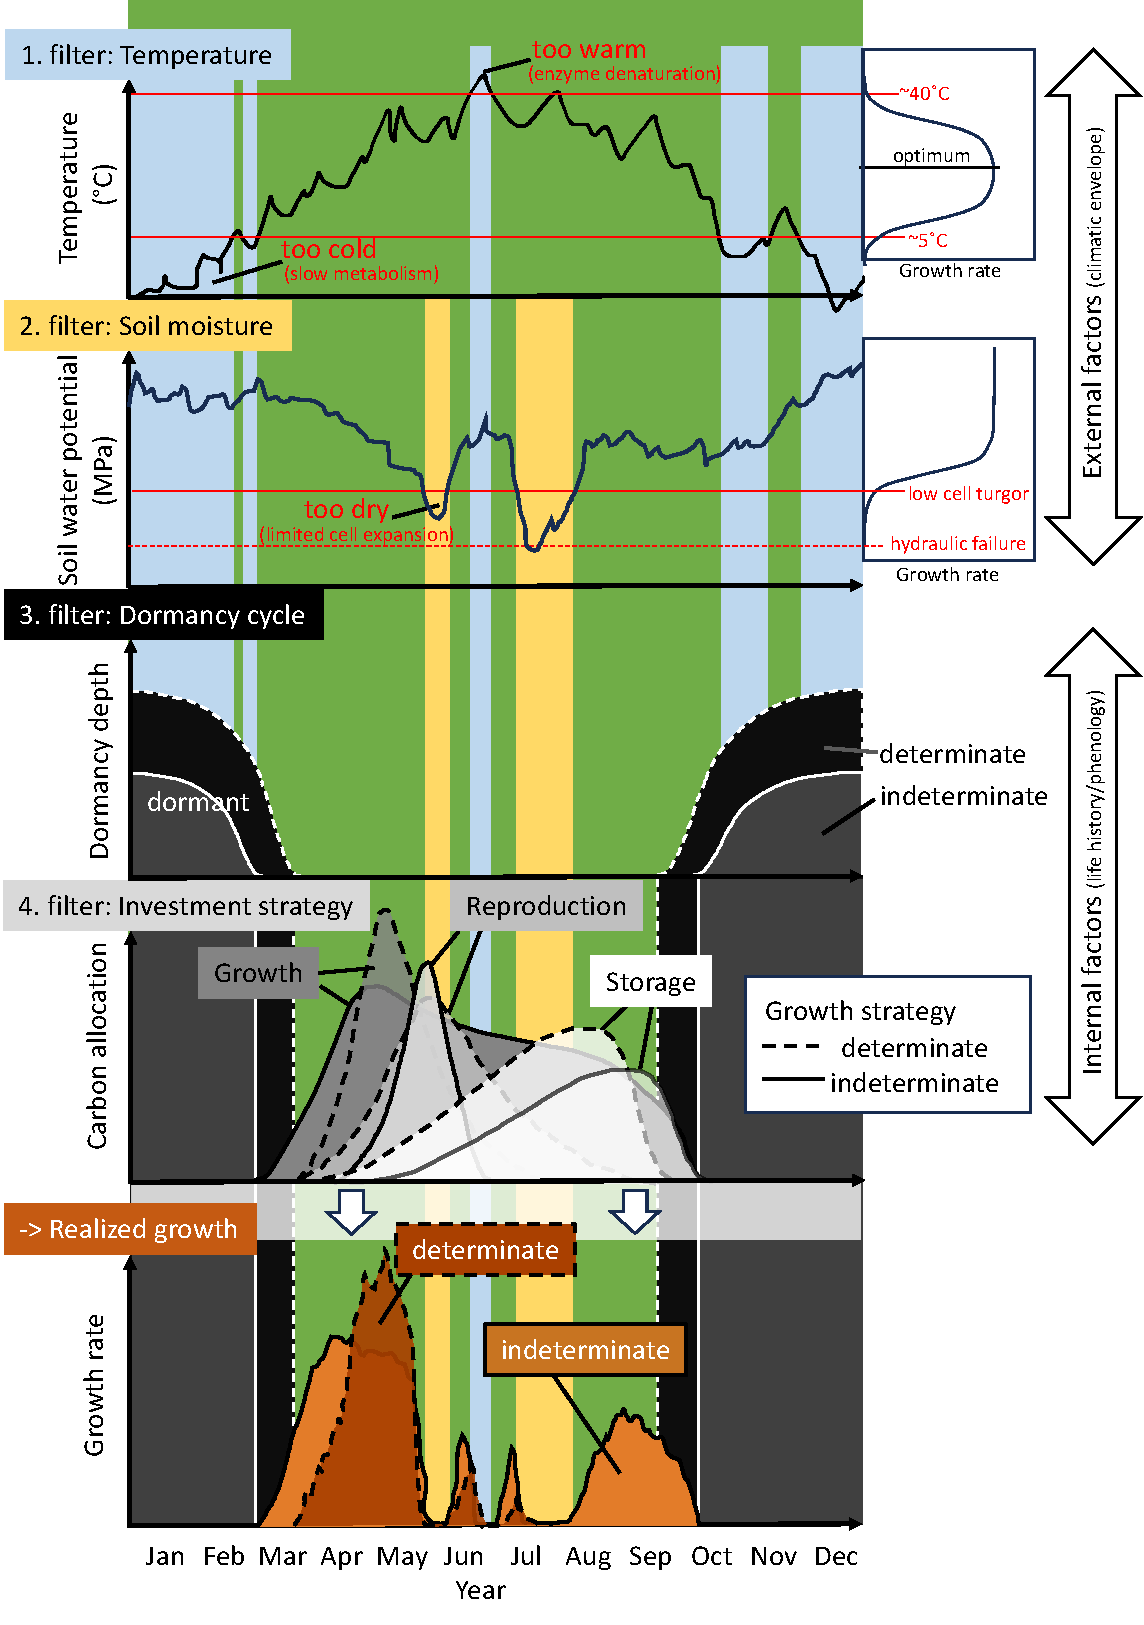
\includegraphics[width=0.9\textwidth]{Fig_1_V6.pdf} 
								\caption{Schematic overview of the discrepancy between the potential growing season and the effectively realized vegetative growth. Environmental factors like temperature and soil moisture, exceeding growth-promoting thresholds can be seen as filters that narrow the window of opportunity available for vegetative growth. The species-specific life history cycle (phenology) can impose another filter by dictating a dormancy cycle and prioritizing developmental processes other than vegetative growth (e.g. flowering, fruit maturation and storage). }
								\label{fig:fig_1xxx}
							\end{figure}

	
\section*{The concept of (in)determinate growth}
	\subsection*{Fixed size or life-long growth}
	The topic of growth strategies and habits has a long history in science, spanning the fields of genomics, physiology and ecology across the animal and plant kingdoms. At its core lays the concept of determinacy---the classification of organisms to either reach a fixed size with adulthood or to continue to grow throughout their lifetime. Like mollusks, fish and reptiles, plants add to their primary bodies as long as they live and are therefore considered `indeterminate growers' \citep{ejsmondHowTimeGrowth2010}. Various terms emerged to describe this fundamental phenomenon at different spacial and temporal scales, e.g. from a cell to an organism and from a season to a whole lifetime \citep{mcdanielInductionDeterminationDevelopmental1992a, karkachTrajectoriesModelsIndividual2006}. \\

	\subsection*{Full abortion or temporal suspension of the meristem}
	In annual plants, growth ends with the production of flowers to form fruits and seeds: a signal in the apical meristem causes a sudden switch in resource investment from vegetative growth to building a reproductive structure with no point of return, ringing in the end of its life-cycle \citep{poethigPhaseChangeRegulation2003, huijserControlDevelopmentalPhase2011}. An axis that will irreversibly abort meristematic competency and end in a flower or other structure is considered `determinate' \citep{barthelemyPlantArchitectureDynamic2007}. In the case of trees, flowers are build on lateral shoots/buds to ensure the continues expansion of the vegetative structure and the seasonal production of offsprings. However, the term "determinate growth" also refers to a temporal suspension of the meristem, which leads to a time lag between the formation of tissue and its expansion. \citep{kozlowskiSeedGerminationOntogeny2012, halleTropicalTreesForests1978}. 
	
	\subsection*{Pre- or neo-formation of tissue}
	Commonly, trees prebuild their new shoot increments in the previous year, overwintering in hardened buds to be `ready-to-go' when spring arrives. Once the entire canopy is unfolded within a few days to weeks (in the case of deciduous trees) some species suspend their primary growth activity by hormonal suppression of the apical meristems for the rest of the season \citep[paradormancy,][]{langEndoParaEcodormancy1987}.  Other species, however, continue to produce new tissue ontop/beyond of the preformed one, in some cases stretching their growth period far into autumn until low temperature force them to stop. In essence, determinacy in trees as we use it from here on, refers to the ability to:\\
	a) preform tissue as a future investment that is ready to be deployed in spring with no further primary growth thereafter (determinate strategy)\\
	b) maintain a somewhat constant growth activity (or activity bursts) by forming new tissue during the current growing season (indeterminate strategy)\\

While this concept is often presented as dichotomous \citep{kozlowskiGrowthControlWoody1997, lechowiczWhyTemperateDeciduous1984a}, but see \citealp{kikuzawaLeafSurvivalWoody1983, damascosBudCompositionBranching2005}), with species exhibiting either one extreme or the other, they more likely exist along a gradient with numerous intermediate forms. For example many oak species considered determinate growers, exhibit a second flush and many species gradually become more determinate as they mature \citep{borchertConceptJuvenilityWoody1976, heuretOntogeneticTrendsMorphological2006}.
	
								\begin{figure}
								\centering
								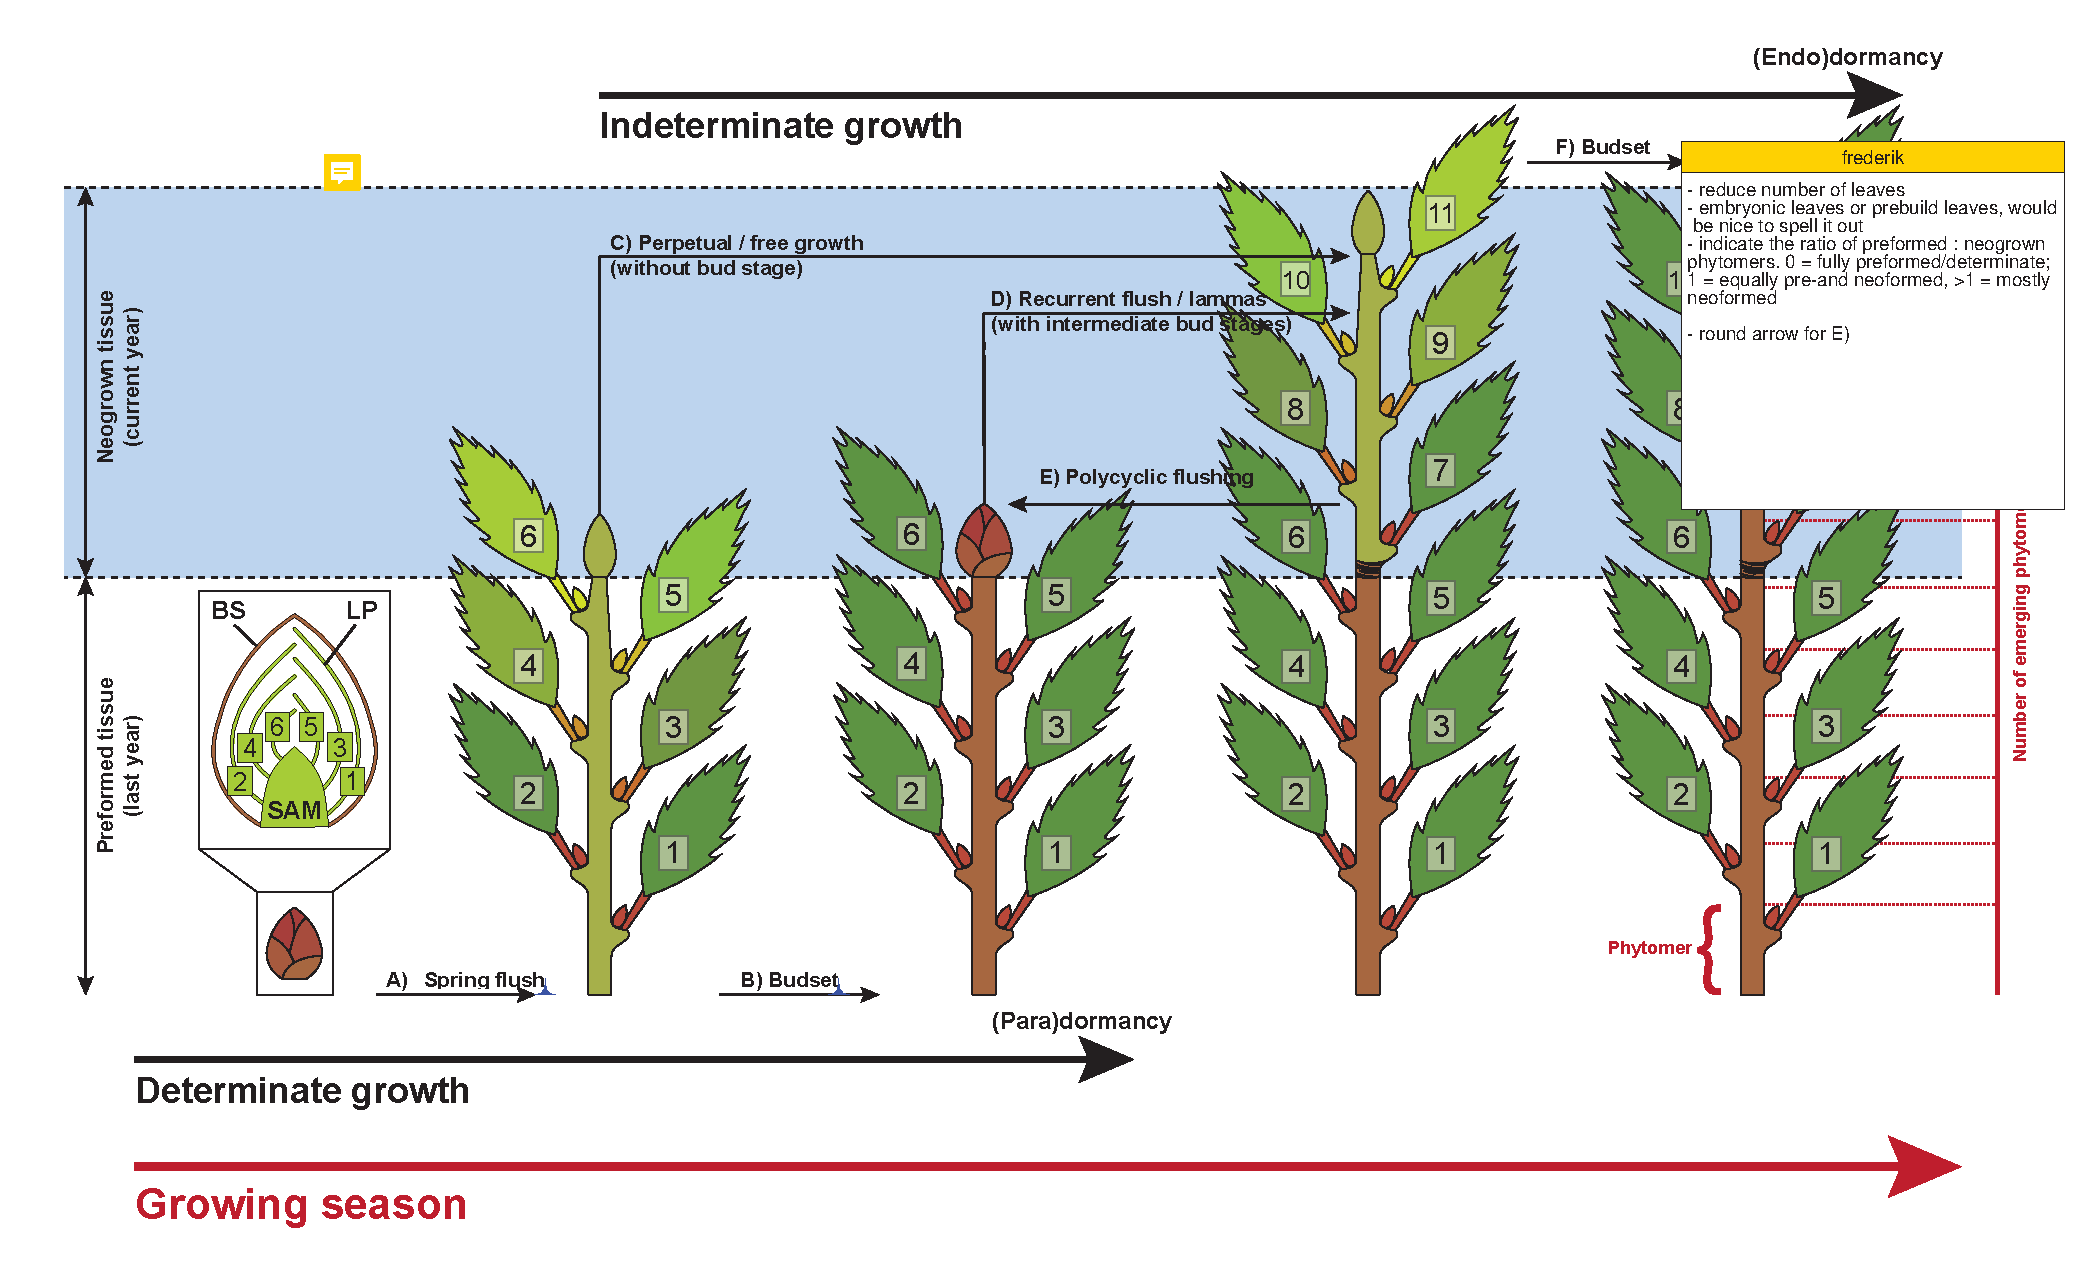
\includegraphics[width=1.1\textwidth]{determinismFigure_FB.pdf} 
								\caption{Determinate and indeterminate growth within one growing season. Commonly all tree species deploy buds during their first spring flush from prebuild and overwintering leaf primordia (A). Determinate growing species set bud (B) that are under hormonal suppression to sustain any further activity of the shoot apical meristem (paradormancy). Indeterminate growing species continue to produce new tissue directly (C) or through one (D) to several (E) intermediate bud stage(s). Finally all species set their bud (F) and enter full dormancy (endodormancy). Shoot apical meristem (SAM); Bud scale (BS); leaf primordia (LP). The basic unit of a shoot is the phytomer which is composed of a node, a leaf, the axillary bud and an internode.}
								\label{fig:fig_2xxx}
								\end{figure}
%	\begin{mytextbox}[]
	%	\subsection*{Box 1: Definitions)}
	%	\textbf{Growth habit}: The genetic tendency of a plant to form a characteristic habitus (shape, height, form) with a particular branching and growth pattern. \\
%		\textbf{determinate growth}: a growth pattern characterized to stop at a predefined size. Commonly, the apical bud culminates in an inflorescence, halting the production of any additional leaves or buds. In trees this terms specifies the short duration of extension growth in spring with no further activity of the apical meristem.\\
		%\textbf{indeterminate growth}: a growth pattern characterized by continuous growth (leaves, buds or flowers) throughout their life or as long as condition remain favourable. This is possible because the apical meristems always remain vegetative and flowers are restricted to lateral meristems. In trees this refers to the continuous shoot elongation throughout the growing season.\\
		%\textbf{Neogrowth}: Growth that occurs on top of preformed tissue due to the more or less continuous activity of the shoot apical meristem. Several forms occur depending on whether growth occurs continuously or in bursts.\\
		%\textbf{Perpetual/Continuous/free/sustained growth}: the constant production of new tissue without interruptions of bud stages.\\
		%\textbf{Polycyclic growth:} Growth occurs in bursts after the initiation of leaf primordia inside buds.  \\
		%\textbf{Second flush:} Growth form of species in which one additional cohort of buds is build and deployed during the current growing season. In the German literature this is often termed ‘Johannitrieb’ since the flush often occurs around the summer solstice. Also ‘lammas growth’ is a common term for an additional flush (lammas = loaf mass; old English for the holy communion typically to celebrate the first harvest).\\
		
	%\end{mytextbox}

	
\section*{Control mechanisms of (in)determinacy}
Although a century of studying growth habits has passed we still have very little understanding of when and why trees exhibit a certain degree of (in)determinacy in their growth strategy. To a large extent this is probably due to the variable environmental conditions within and between years as well as among sites and individuals that complicates the separation of internal from external factors influencing or driving primary growth and for that matter other meristematic activity.

There is indeed evidence that under favorable conditions, particularly under high soil moisture availability throughout the growing season, the time of shoot elongation is extended, e.g. by enabling an additional flush REF. Such findings indicate that shoot growth may come to a halt because the demand for water to support an increasing leaf area cannot be met. Hence an imbalance of the root:shoot ratio under a given water status of the plant can suppress primary growth as was shown experimentally by \citet{borchertSimulationRhythmicTree1973}. By the same mechanism, many species are able to produce new shoots to rebuild the canopy after a considerable loss of leaf area due to herbivory or damaging spring frosts REF. 

One might conclude that the environment can completely flip a species' strategy---but research shows that this is not the case REF.  While many species have shown a certain plasticity of the apical shoot meristem, they still exhibit distinct growth patterns when environmental conditions remain favorable and disturbances are excluded REF. Hence, there must be an underlying internal program that sets the potential of how trees grow and explains the variation of growth habits among species we observe in the same environmental conditions (see Table XX for a list of species and their main growth strategy). 

latitudinal gradients and population differences within a species...Sally?
	
what are the fundamental trade-offs? 
do indeterminate species grow faster and have a shorter life span? hence faster turnover?

both growth strategies are successful and co -occur in communities
indeterminate species are often early successional ones \citep{marksRelationExtensionGrowth1975, boojhGrowthStrategyTrees1982}
ontogeny as another control mechanism: becoming more conservative and determinate with age	

	...but will both still be successful with CC?
	
\section*{The role of (in)determinacy with climate change}
Climate change is extending the growing season length while at the same time increasing the risk for severe drought \citep{haoChangesSeverityCompound2018} and presumably also late spring frost events in many regions worldwide \citep{zohnerLatespringFrostRisk2020}. How are these potential benefits and threads linked to a species strategy, specifically to the degree of determinacy? Which strategy profits most from an extended growing season length and which one is flexible enough to rearrange their phenological cycle to withstand increased environmental stress. And which one comes with more biomass production and C sequestration? The role of primary growth has been widely neglected to help answering these questions, although it sets photosynthesis biomass and overall source capacity \citep{girardPolycyclismFundamentalTree2011}. We propose that the degree of determinacy is an important trait largely controlling the responses of trees in a future climate illustrated in Figure \ref{fig:fig_4xxx}. \\

Spring warming has advanced the onset of leaf emergence by up to a month compared to pre-industrial times \citep{vitasseGreatAccelerationPlant2022b}. In contrast autumn phenology of growth and leaf senescence has not delayed as one could predict from environmental conditions \citep{zaniIncreasedGrowingseasonProductivity2020b, zohnerEffectClimateWarming2023}. In fact, the phenological sequence is observed to shift more as a whole towards spring \citep{keenanTimingAutumnSenescence2015b}, not necessarily leading to increased biomass production during longer growing seasons \citep{zaniIncreasedGrowingseasonProductivity2020b}. We hypothesize that only determinate growing species shift their growth in such a way with minimal changes in overall productivity. In contrast, indeterminate growing species are able to extend their growing period in both directions, potentially leading to an increased productivity in a future climate (Figure \ref{fig:fig_4xxx}). \\

The flexible growth strategies of indeterminate species that help them exploit longer seasons, could also increase their exposure to extreme climatic events. Indeterminate species are often among the first to leaf-out and among the last to shed their leaves \citep{marksRelationExtensionGrowth1975, boojhGrowthStrategyTrees1982}---occasionally as a result of first freezing events in autumn. In addition, a substantial part of their growth period falls into summer with increased risk of drought (Figure \ref{fig:fig_4xxx}). Therefore, we hypothesize that the conservative strategy of determinate growing species largely escape from unfavorable growing conditions by placing their growth activities between the last spring frost and the increasing water shortages in summer, with relatively ample safety margins. As a consequence productivity shows little between year variation and will largely remain constant in a future climate. However, once hit by an extreme event, determinate growing species might not recover easily. Even if the leaves are shed to prevent further damage, the loss of the canopy, which is rarely replaced after the summer in determinate species, will prevent replenishment of the reserve pools and ultimately reduce fitness. In contrast, the flexible growth schedule of indeterminate growing species may allow to 1) produce tissue better adapted to harsh environmental conditions as it is formed in the current season and 2) catch up and compensate later in the season by another productivity boost. Taking advantage of a `second growing season' after summer drought was indeed shown for pines in the mediterranean climate through polycyclic flushing---a form of indeterminate growth \citep[Figure \ref{fig:fig_2xxx}]{girardPolycyclismFundamentalTree2011}. \\

We argue that new opportunities and challenges for trees with climate change will increasingly disrupt their phenological cycle, favoring species who are more plastic in rearranging their activities by resuming growth, reproduction and/or storage filling later in the year, thereby recovering from and compensating for some stress-induced damages and losses. Future climate will therefore likely intensify the competition among co-occurring species and might re-assemble forest communities increasingly composed of species adopting an indeterminate growth strategy.
	
	
								\begin{figure}
								\centering
								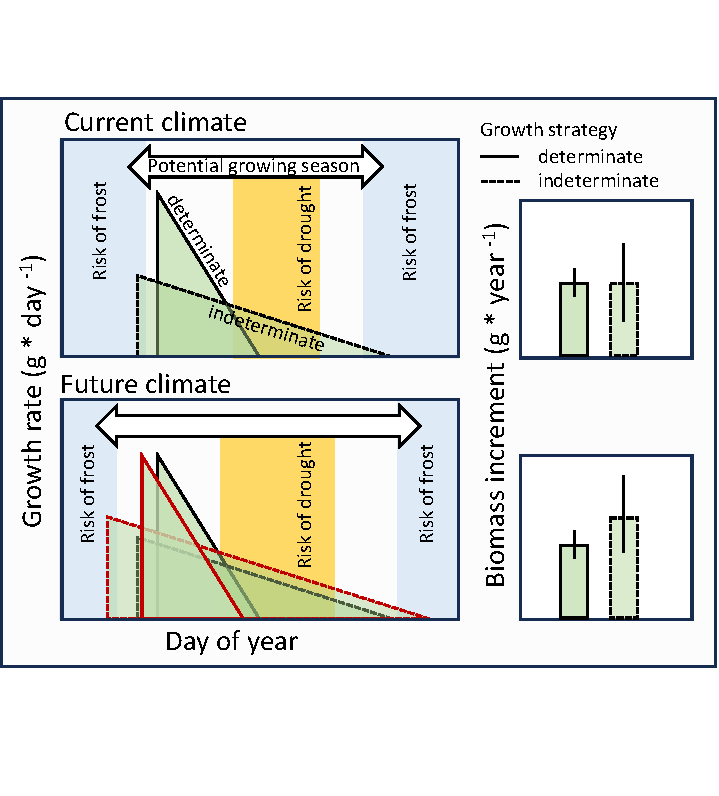
\includegraphics[width=0.9\textwidth]{Fig_4_V1.pdf} 
								\caption{Hypothesized predictions of growth rates under current and future climate for determinate and indeterminate growing species. Note that the indeterminate strategy is more exposed to the risk of frost and drought events while the determinate strategy condenses most growth within a rather safe period. In the current climate the indeterminate strategy is in balance with benefiting from the full climatic growing season in some years with some drawback in other years, resulting in the same mean yearly biomass increment, but with a higher variation; right box). In a future climate the indeterminate strategy might benefit exceedingly from longer growing seasons, resulting in an overall higher mean annual biomass increment compared to determinate growers.}
								\label{fig:fig_4xxx}
							\end{figure}
	\pagebreak
\section*{Future directions}
We argue that incorporating plant determinacy into our models of forest dynamics could provide better answers to major questions. When and how much is growth and therefore carbon sequestration most impacted by climate extremes and longer growing seasons likely depends on the ratio of indeterminate to determinate growing species in a forest community. These two strategies, and better understanding them will also help to reveal the potentials and limits of trees to adapt in a future climate.

Specifically, how much degree of (in)determinacy allows to escape periods of increased risk of environmental stress while being versatile enough to resume metabolic activities to repair damaged structures, restore reserves and eventually compensate for previous losses during the same season. Assessing the trade-off between buffering extreme events and exploiting a longer growing season will likely contribute to our understanding of how forest communities will assemble over the course of this century.\\

Going forward, we need to identify the plasticity of the trait of exhibiting indeterminate growth under different environmental conditions and the genetic programming of a species and to what extend the latter prioritizes the former. Namely, across species and populations and involving different fields from genomics to physiology and ecology. Moreover, how much indeterminate growth will impact carbon sequestration, in part depends on understanding how universal the concept of (in)determinacy holds across tissue and meristem types. 

\subsection*{(In)determinacy beyond leaf tissue} 
Although (in)determinate growth is mainly associated with the activity of the shoot apical meristem, a similar pattern or concept might be found in the cambium as well to ensure a timely switch from vegetative growth to reproductive and storage investments. In fact, also cambial cells produce several cohorts of precursor cells with differentiation being completed at a much later stage only \citep{valdovinos-ayalaSeasonalPatternsIncreases2022}. Hence the number of initial cells divided at the beginning largely determines the amount of total xylem produced \citep{lupiXylemPhenologyWood2010}. In this case, primary growth reflects or at least influences the overall growth performance of an individual, integrated across all above-ground meristems. The low predictive power to estimate the end of wood formation in autumn reported by several studies \citep{buttoComparingCellDynamics2020} indeed points to a mechanism that stem growth in many tree species ceases despite of ongoing favorable conditions and a green canopy \citep{arendStemGrowthPhenology2024}.\\

Regarding below-ground meristems, roots seem to follow a much more opportunistic strategy with indeterminate growth potentially occurring throughout the year. Warming experiments using rhizotrones have shown that roots can grow even in mid-winter if temperature allow it \citep{lyfordControlledGrowthForest1966}, suggesting that roots do not enter a state of dormancy \citep{radvilleRootPhenologyChanging2016}. To what extend asynchronous between above and below-ground meristems occur as a result of different tissue temperatures, root:shoot imbalances or genetically fixed investment strategies remain unresolved \citep{abramoffAreBelowgroundPhenology2015, makotoSynchronousAsynchronousRoot2020}.\\

 Future studies should therefore link the temporal dynamics of primary (apical and root) and secondary (cambial) meristems. Correlating annual tree rings with shoot increments could reveal such a common pattern, if accounting for when inter-annual shoot segments (phytomers) were produced, e.g. separating preformed from neo-grown tissue (REF Günter?). Revealing the patterns of when different meristems are active will likely contribute to a theoretical framework of temporal carbon allocation dynamics.

							\begin{figure}
							\centering
							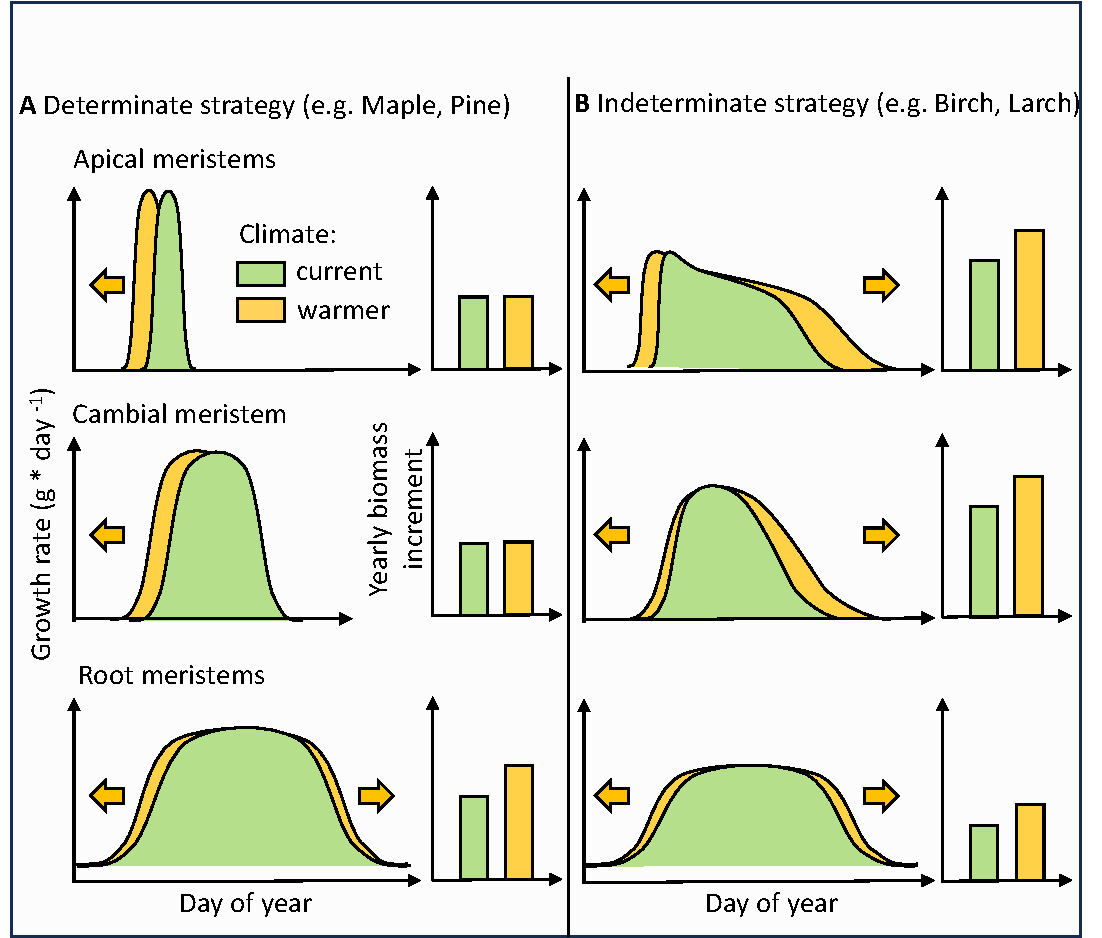
\includegraphics[width=0.9\textwidth]{Fig_3_V3.pdf} 
							\caption{Hypothesized predictions of growth rates for the three major meristems (apical, cambium and root) classes of trees under current and warmer climates following an extreme determinate (A) and indeterminate (B) growth strategy. The area under the curve is summarized as yearly biomass increment in the respective bar-plot. Arrows indicate the shift of growth phenology under warmer climate conditions. Root meristems appear to be purely temperature-opportunistic for both strategies, even growing during warm winter spells. The indicated genera were observed to showcase the illustrated trends. The responses of these two contrasting growth strategy might apply not only to different tree species but also within a population (e.g. along environmental gradients) and even within an individual as it transitions from the juvenile to the adult stage (ontogeny).}
							\label{fig:fig_3xxx}
						\end{figure}

	\subsection*{Evolution of (In)determinacy}
	Understanding how universally tissues within species are formed determinately or indeterminately could provide insight into the evolution of this trait, which could be aided by cross-species analyses. Both growth forms seem to occur across most species of the same genera or clade and hence, appear to have evolved repeatedly in different groups, making it difficult to speculate on which strategy is ancestral \citep[but see][]{hariharanIndeterminateGrowthCould2016} and how rapidly (in)determinacy can evolve. As data on which species are determinate or indeterminate accumulates, such analyses could potentially provide rapid insights into this, and also aid forecasting for unsampled species. Assigning species as determinate or indeterminate, however, may be slow if the trait is actually better considered as continuous. 
	gene/hormones ?
	
	\subsection*{Metrics of (In)determinacy}
	To address these questions we need better metrics to quantify the degree of determinacy, moving beyond a dichotomous classification system. We propose several metrics from best to acceptable, with increasing spatial scale: \\
	
	(1) The ratio of the number of leaves at the end of the season to the initial number of leaf primordia in buds at the start of the season provides a measure of (in)determinacy. Values above one indicate an increasing degree of indeterminate growth. Although this metric was already described over a century ago by \citet{mooreStudyWinterBuds1909}, its application has been limited to few studies exploring specific regions only \citep{damascosBudCompositionBranching2005, kikuzawaLeafSurvivalWoody1983, guedonRelativeExtentsPreformation2006}. Moreover, to reveal the endogenous potential of indeterminate growth, individuals have to be grown under constant favorable conditions (e.g. unlimited soil moisture).\\
	
	(2) Direct measures of shoot elongation (height increments) and/or xylogenesis (micro-cores) at high temporal resolution (e.g. bi-weekly) to assess the temporal dynamics of apical and cambial activity. Especially wood anatomical observations ensure the distinction of cell formation and their subsequent enlargement and development REFS\\
	
	(3) As a proxy for the above, dendrometers provide insights of xylem and phloem formation at high temporal resolution. Although obtained measurements are a mixture of several processes, it allows to identify the tree water deficits and related growth reductions \cite{etzoldNumberGrowthDays2021, zweifelWhyTreesGrow2021}. \\
	
	(4) Using observations of 'second flushes' in large databases (e.g. US national forest network). \\%@Lizzie: any references here and examples/specifics of how to use it?
	
	(5) Patterns and fluctuations of canopy growth can be detected from drones or satellites using LiDAR or various spectral techniques. The temporal trend of canopy greenness over the growing season can reveal investment strategies integrated across entire ecosystems and vast areas. As a recent example, \citet{mengConsistentTimeAllocation2024} found that time allocation between vegetation green-up (from start of the growing season to its peak) and vegetation senescence (between peak and end of season) remained constant despite substantial differences in growing season lengths and degree of warming in temperate ecosystems across the northern hemisphere.  %Could be also a section "Evidence for internal growth control" 

	

	
\section*{Acknowledgments}
	This text emerged from a grant of the Swiss National Foundation to F.B. (grant number P500PB\textunderscore 210943). We thank J. Ngo for designing figure 2 and XXXX
	
	

	
	\pagebreak
	

	\newpage
\section*{stuff I did't find place yet}
Ontogeny: 
the preformation of leaves inside the seed may be a better strategy than seed mass \citep{silvaCouldPresencePreformed2023}


Deciduous tree species have a higher number of leaf primordia inside their buds than evergreen species in the Cerrado (Brazil). 
	
If experiments are conducted in conditions with unlimited soil moisture and under similar temperature regimes, then the dynamics of growth responses can be comparable among species and reveal their potential in deploying indeterminate growth. Under natural conditions with common soil moisture and associated turgor limitations it is currently hard to tell if trees cease growth because of a response to the environment or because of switches in resource allocation. 

 Grow fast die young...
 
 Even in grasslands an earlier onset of growth is associated with an earlier stop under climate warming \cite{mohlGrowthAlpineGrassland2022a}
	
	
	must include: 
	
	\cite{iwasaOptimalGrowthSchedule1989}
	
	
	
	Shoot growth patterns do not only tell us something about the plant architecture and the strategy of space exploitation, but may reveal also patterns of the whole-plant dynamic and potential of growth and carbon sequestration.
	
	unit of extension vs. unit of morphogenesis: Perhaps state somewhere that we commonly only observe the extension pattern while patterns of organogenesis remain hidden. 
	
	\cite{barthelemyPlantArchitectureDynamic2007}: determinate growth: irreversable transformation of the apical meristem (flowering or other structures, apical death/abscission)
	indeterminate growth: functioning of the apical meristems remains intact (but may have periods of rest)
	 
	 
	
	\newpage
	
	\bibliography{refs_determinism}
	\bibliographystyle{ecolett}
	
	
	
\end{document}






